\documentclass[]{gshs_exam_S}

\usepackage{lipsum}
\usetikzlibrary{patterns,decorations.pathmorphing}
\usepackage{bm}

\usepackage{tikz-3dplot}


\makeatletter
\myyear{2018}\let\MyYear\@myyear %학년도
\semester{1}\let\Semester\@semester %학기
\exams{1차 지필평가}\let\Exams\@exams %1차,2차 지필평가
\subject{미적분학II}\let\Subject\@subject %과목명
\credits{3} %학점
\pfscore{100} %만점
\examtime{120분} %시험시간
\examiner{한상현} %출제
\reviewer{강형종} %검토
\makeatother

\begin{document}

\maketitle

%%% page 1 %%%
\begin{multicols*}{2}
\noindent\fbox{\parbox{0.98\columnwidth}{\vspace*{-0.6em}
\begin{enumerate}[leftmargin=5.5mm,label=※]
\item 문항에 따라 배점이 다르므로 각 물음의 끝에 표시된 배점을 참고하시오.\\[-1.6em]
\item 서술형 ( 80 )점 포함, 논술형 ( 20 )점 포함
\end{enumerate}\vspace{-0.6em}}}\vspace{1em}

\begin{questions}
\extrawidth{8.1em}
%%% Problem 1 %%%
\addpoints
\question Suppose that $\mathbf{u}$, $\mathbf{v}$, and $\mathbf{w}$ are vectors in space, so that they determine a parallelepiped as in the Figure below. Justify your answers to the following questions.\droptotalpoints
\begin{center}
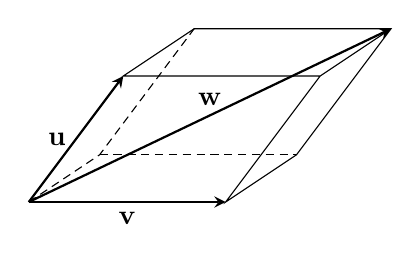
\begin{tikzpicture}
\def\ux{1.2}\def\uy{1.6}
\def\vx{2.5}\def\vy{0}
\def\wx{0.9}\def\wy{0.6}
\draw[-stealth,thick] (0,0) -- (\ux,\uy) node[pos=0.5,left] {$\mathbf{u}$};
\draw[-stealth,thick] (0,0) -- (\vx,\vy) node[pos=0.5,below] {$\mathbf{v}$};
\draw[-stealth,thick] (0,0) -- ({\ux+\vx+\wx},{\uy+\vy+\wy}) node[pos=0.5,above] {$\mathbf{w}$};
\draw ({\ux+\vx},{\uy+\vy}) -- ++(-\ux,-\uy) -- ++(\wx,\wy) -- ++(\ux,\uy) -- ++(-\vx,-\vy) -- ++(-\wx,-\wy) -- ++(\vx,\vy) -- ++(\wx,\wy);
\draw[densely dashed] (0,0,0) -- ++(\wx,\wy) -- ++(\ux,\uy);
\draw[densely dashed] (\wx,\wy) -- ++(\vx,\vy);
\end{tikzpicture}
\end{center}
\begin{parts}
\part[4] \ssh\ Give formulas for the surface area and the volume of the parallelepiped in terms of $\mathbf{u}$, $\mathbf{v}$, and $\mathbf{w}$.\droppoints
\vspace{2em}
\part[4] \ssh\ Use furmulas in (1) to find the surface area and the volume of the parallelepiped when
\[
\mathbf{u}=\mathbf{i}+\mathbf{j}+2\mathbf{k},\quad\mathbf{v}=\mathbf{j}+\mathbf{k},\quad\mathbf{w}=-2\mathbf{i}+\mathbf{j}+3\mathbf{k}.
\]
\droppoints
\end{parts}

\vspace*{\fill}
\columnbreak

%%% Problem 2 %%%
\addpoints
\question Justify your answers to the following questions.\droptotalpoints
\vspace{2em}
\begin{parts}
\part[3] \ssh\ Find an equation of the plane $M$ through the point $(2,2,0)$ that is parallel to the vector $\mathbf{i}+\mathbf{j}+\mathbf{k}$ and perpendicular to the plane $x+2y+6z=6$.\droppoints
\vspace{2em}
\part[3] \ssh\ Find parametric equations for the line $L$ of intersection of the plane $x+2y+6z=6$ and the plane $M$ in (1).\par\droppoints
\vspace{2em}
\part[3] \ssh\ Let $P$ be a plane in space and let $\mathbf{v}$ be a vector. The vector projection of $\mathbf{v}$ onto the plane $P$, $\mathrm{proj}_P \mathbf{v}$, can be defined informally as follows. Suppose the sun is shining so that its rays are normal to the plane $P$. Then $\mathrm{proj}_P \mathbf{v}$ is the ``shadow'' of $\mathbf{v}$ onto $P$. If $P$ is the plane $x+2y+6z=6$ and $\mathbf{v}=\mathbf{i}+\mathbf{j}+\mathbf{k}$, find $\mathrm{proj}_P \mathbf{v}$.\droppoints
\end{parts}

\end{questions}
\end{multicols*}


%%% page 2 %%%
\begin{multicols*}{2}
\begin{questions}\extrawidth{8.1em}\setcounter{question}{2} %이전 페이지 마지막 문항 번호 입력

%%% Prob 3 %%%
\addpoints
\question Justify your answer to the following questions.\droptotalpoints
\vspace{2em}
\begin{parts}
\part[3] \nsh\ Show that if $\mathbf{u}$, $\mathbf{v}$, and $\mathbf{w}$ are differentiable vector functions of $t$, then
\[
\frac{d}{dt}(\mathbf{u}\cdot\mathbf{v}\times\mathbf{w})=\frac{d\mathbf{u}}{dt}\cdot\mathbf{v}\times\mathbf{w}+\mathbf{u}\cdot\frac{d\mathbf{v}}{dt}\times\mathbf{w}+\mathbf{u}\cdot\mathbf{v}\times\frac{d\mathbf{w}}{dt}.
\]
\droppoints
\part[3] \ssh\ Show that
\[
\frac{d}{dt}\left(\mathbf{r}\cdot\frac{d\mathbf{r}}{dt}\times\frac{d^2 \mathbf{r}}{dt^2}\right)=\mathbf{r}\cdot\left(\frac{d\mathbf{r}}{dt}\times\frac{d^3 \mathbf{r}}{dt^3}\right).
\]
\droppoints
\end{parts}

\vspace*{\fill}
\columnbreak

%%% Prob 4 %%%
\addpoints
\question A baseball is hit when it is $1\,\mathrm{m}$ above the ground. It leaves the bat with initial speed of $40\,\mathrm{m/s}$, making an angle of $30^\circ$ with the horizontal. At the instant the ball is hit, an instantaneous gust of wind blows in the horizontal direction directly opposite the direction the ball is taking toward the outfield, adding a component of $-3\mathbf{i}\,\mathrm{m/s}$ to the ball's initial velocity. Justify your answers to the following questions. (Use the acceleration due to the gravity as $g=10\,\mathrm{m/s^2}$.\par\droptotalpoints
\vspace{2em}
\begin{parts}
\part[3] \ssh\ Find a vector equation (position vector) for the path of the baseball.\droppoints
\vspace{2em}
\part[3] \ssh\ How high does the baseball go, and when does it reach maximum height?\droppoints
\vspace{2em}
\part[3] \ssh\ Assuming that the ball is not caught, find its range and flight time.\droppoints
\end{parts}

\end{questions}
\end{multicols*}

%%% page 3 %%%
\begin{multicols*}{2}
\begin{questions}\extrawidth{8.1em}\setcounter{question}{4}

%%% Problem 5 %%%
\addpoints
\question Justify your answers to the following questions.\droptotalpoints
\vspace{2em}
\begin{parts}
\part[4] \nsh\ Show that the curvature $\kappa_1$ of the smooth curve given by the twice-differentiable vector function $r$ is
\[
\kappa_1 (t)=\frac{|\mathbf{r}^\prime (t)\times\mathbf{r}^{\prime\prime} (t)|}{|\mathbf{r}^\prime (t)|^3}.
\]
\droppoints
\vspace{2em}
\part[4] \ssh\ Use (1) to show the curvature $\kappa_2$ of the smooth curve in polar coordinates described by twice-differentiable function $r=f(\theta)$ is
\[
\kappa_2 (\theta)=\frac{\left| r^2 +2\left(\dfrac{dr}{d\theta}\right)^2 -r\dfrac{d^2 r}{d\theta^2}\right|}{\left[ r^2 +\left(\dfrac{dr}{d\theta}\right)^2 \right]^{3/2}}.
\]
\droppoints
\end{parts}

\vspace*{\fill}
\columnbreak

%%% Problem 6 %%%
\addpoints
\question The following formulas are called the Frenet--Serret formulas. ($s$ is an arc length parameter for the curve.) Justify your answers to the following questions.\droptotalpoints
\vspace{1.5em}
\noindent\fbox{
\parbox{0.95\linewidth}{
\begin{itemize}
\item[(a)] $\dfrac{d\mathbf{T}}{ds}=\kappa\mathbf{N}$
\item[(b)] $\dfrac{d\mathbf{N}}{ds}=-\kappa\mathbf{T}+\tau\mathbf{B}$
\item[(c)] $\dfrac{d\mathbf{B}}{ds}=-\tau\mathbf{N}$
\end{itemize}
}}
\vspace{1.5em}
\begin{parts}
\part[4] \nsh\ Show that
\[
\textrm{(b)}\ \ \frac{d\mathbf{N}}{ds}=-\kappa\mathbf{T}+\tau\mathbf{B}.
\]
\droppoints
\vspace{2em}
\part[4] \nsh\ Use (a) and (b) to show that
\[
\mathbf{B}=\frac{\mathbf{r}^\prime (s)\times\mathbf{r}^{\prime\prime} (s)}{|\mathbf{r}^{\prime\prime} (s)|}.
\]
\droppoints
\end{parts}

\end{questions}
\end{multicols*}


%%% page 4 %%%
\begin{multicols*}{2}
\begin{questions}\extrawidth{8.1em}\setcounter{question}{6}

%%% Problem 7 %%%
\addpoints
\question Answer to the following questions. \droptotalpoints
\vspace{2em}
\begin{parts}
\part[5] \nsh\ Prove the statement using the $\epsilon$, $\delta$ definition of limit.
\[
\lim_{(x,y)\rightarrow(0,0)} 3y^2 \frac{x^2 -y^2}{x^2 +y^2}=0
\]
\droppoints
\vspace{2em}
\part[4] \ssh\ Find the limit, if it exists, or show that the limit does not exist. Justify your answer.
\[
\lim_{(x,y)\rightarrow(0,0)} xy^2 \sin\frac{1}{x^2 +y^2}
\]
\droppoints
\end{parts}

\vspace*{\fill}
\columnbreak

%%% Problem 8 %%%
\addpoints
\question Justify your answers to the following questions.\droptotalpoints
\vspace{2em}
\begin{parts}
\part[5] \ssh\ Let
\[
f(x,y)=\begin{cases}\dfrac{xy^2}{x^2 +y^4}&(x,y)\ne(0,0)\\0&(x,y)=(0,0)\end{cases}.
\]
Show that $f_x (0,0)$ and $f_y (0,0)$ exist, but $f$ is not differentiable at $(0,0)$.\droppoints
\vspace{2em}
\part[5] \ssh\ Let
\[
f(x,y)=\begin{cases}(x^2 +y^2 )\sin\dfrac{1}{\sqrt{x^2 +y^2}}&(x,y)\ne(0,0)\\0&(x,y)=(0,0)\end{cases}.
\]
Show that $f$ is differentiable at $(0,0)$, but $f_x$ is not continuous at $(0,0)$.\droppoints
\end{parts}

\end{questions}
\end{multicols*}


\end{document}